\documentclass[]{article}
\usepackage{lmodern}
\usepackage{amssymb,amsmath}
\usepackage{ifxetex,ifluatex}
\usepackage{fixltx2e} % provides \textsubscript
\ifnum 0\ifxetex 1\fi\ifluatex 1\fi=0 % if pdftex
  \usepackage[T1]{fontenc}
  \usepackage[utf8]{inputenc}
\else % if luatex or xelatex
  \ifxetex
    \usepackage{mathspec}
  \else
    \usepackage{fontspec}
  \fi
  \defaultfontfeatures{Ligatures=TeX,Scale=MatchLowercase}
\fi
% use upquote if available, for straight quotes in verbatim environments
\IfFileExists{upquote.sty}{\usepackage{upquote}}{}
% use microtype if available
\IfFileExists{microtype.sty}{%
\usepackage{microtype}
\UseMicrotypeSet[protrusion]{basicmath} % disable protrusion for tt fonts
}{}
\usepackage[margin=1in]{geometry}
\usepackage{hyperref}
\hypersetup{unicode=true,
            pdftitle={Teste de Hipóteses: Introdução},
            pdfauthor={Fernando B. Sabino da Silva},
            pdfborder={0 0 0},
            breaklinks=true}
\urlstyle{same}  % don't use monospace font for urls
\usepackage{color}
\usepackage{fancyvrb}
\newcommand{\VerbBar}{|}
\newcommand{\VERB}{\Verb[commandchars=\\\{\}]}
\DefineVerbatimEnvironment{Highlighting}{Verbatim}{commandchars=\\\{\}}
% Add ',fontsize=\small' for more characters per line
\usepackage{framed}
\definecolor{shadecolor}{RGB}{248,248,248}
\newenvironment{Shaded}{\begin{snugshade}}{\end{snugshade}}
\newcommand{\KeywordTok}[1]{\textcolor[rgb]{0.13,0.29,0.53}{\textbf{#1}}}
\newcommand{\DataTypeTok}[1]{\textcolor[rgb]{0.13,0.29,0.53}{#1}}
\newcommand{\DecValTok}[1]{\textcolor[rgb]{0.00,0.00,0.81}{#1}}
\newcommand{\BaseNTok}[1]{\textcolor[rgb]{0.00,0.00,0.81}{#1}}
\newcommand{\FloatTok}[1]{\textcolor[rgb]{0.00,0.00,0.81}{#1}}
\newcommand{\ConstantTok}[1]{\textcolor[rgb]{0.00,0.00,0.00}{#1}}
\newcommand{\CharTok}[1]{\textcolor[rgb]{0.31,0.60,0.02}{#1}}
\newcommand{\SpecialCharTok}[1]{\textcolor[rgb]{0.00,0.00,0.00}{#1}}
\newcommand{\StringTok}[1]{\textcolor[rgb]{0.31,0.60,0.02}{#1}}
\newcommand{\VerbatimStringTok}[1]{\textcolor[rgb]{0.31,0.60,0.02}{#1}}
\newcommand{\SpecialStringTok}[1]{\textcolor[rgb]{0.31,0.60,0.02}{#1}}
\newcommand{\ImportTok}[1]{#1}
\newcommand{\CommentTok}[1]{\textcolor[rgb]{0.56,0.35,0.01}{\textit{#1}}}
\newcommand{\DocumentationTok}[1]{\textcolor[rgb]{0.56,0.35,0.01}{\textbf{\textit{#1}}}}
\newcommand{\AnnotationTok}[1]{\textcolor[rgb]{0.56,0.35,0.01}{\textbf{\textit{#1}}}}
\newcommand{\CommentVarTok}[1]{\textcolor[rgb]{0.56,0.35,0.01}{\textbf{\textit{#1}}}}
\newcommand{\OtherTok}[1]{\textcolor[rgb]{0.56,0.35,0.01}{#1}}
\newcommand{\FunctionTok}[1]{\textcolor[rgb]{0.00,0.00,0.00}{#1}}
\newcommand{\VariableTok}[1]{\textcolor[rgb]{0.00,0.00,0.00}{#1}}
\newcommand{\ControlFlowTok}[1]{\textcolor[rgb]{0.13,0.29,0.53}{\textbf{#1}}}
\newcommand{\OperatorTok}[1]{\textcolor[rgb]{0.81,0.36,0.00}{\textbf{#1}}}
\newcommand{\BuiltInTok}[1]{#1}
\newcommand{\ExtensionTok}[1]{#1}
\newcommand{\PreprocessorTok}[1]{\textcolor[rgb]{0.56,0.35,0.01}{\textit{#1}}}
\newcommand{\AttributeTok}[1]{\textcolor[rgb]{0.77,0.63,0.00}{#1}}
\newcommand{\RegionMarkerTok}[1]{#1}
\newcommand{\InformationTok}[1]{\textcolor[rgb]{0.56,0.35,0.01}{\textbf{\textit{#1}}}}
\newcommand{\WarningTok}[1]{\textcolor[rgb]{0.56,0.35,0.01}{\textbf{\textit{#1}}}}
\newcommand{\AlertTok}[1]{\textcolor[rgb]{0.94,0.16,0.16}{#1}}
\newcommand{\ErrorTok}[1]{\textcolor[rgb]{0.64,0.00,0.00}{\textbf{#1}}}
\newcommand{\NormalTok}[1]{#1}
\usepackage{graphicx,grffile}
\makeatletter
\def\maxwidth{\ifdim\Gin@nat@width>\linewidth\linewidth\else\Gin@nat@width\fi}
\def\maxheight{\ifdim\Gin@nat@height>\textheight\textheight\else\Gin@nat@height\fi}
\makeatother
% Scale images if necessary, so that they will not overflow the page
% margins by default, and it is still possible to overwrite the defaults
% using explicit options in \includegraphics[width, height, ...]{}
\setkeys{Gin}{width=\maxwidth,height=\maxheight,keepaspectratio}
\IfFileExists{parskip.sty}{%
\usepackage{parskip}
}{% else
\setlength{\parindent}{0pt}
\setlength{\parskip}{6pt plus 2pt minus 1pt}
}
\setlength{\emergencystretch}{3em}  % prevent overfull lines
\providecommand{\tightlist}{%
  \setlength{\itemsep}{0pt}\setlength{\parskip}{0pt}}
\setcounter{secnumdepth}{5}
% Redefines (sub)paragraphs to behave more like sections
\ifx\paragraph\undefined\else
\let\oldparagraph\paragraph
\renewcommand{\paragraph}[1]{\oldparagraph{#1}\mbox{}}
\fi
\ifx\subparagraph\undefined\else
\let\oldsubparagraph\subparagraph
\renewcommand{\subparagraph}[1]{\oldsubparagraph{#1}\mbox{}}
\fi

%%% Use protect on footnotes to avoid problems with footnotes in titles
\let\rmarkdownfootnote\footnote%
\def\footnote{\protect\rmarkdownfootnote}

%%% Change title format to be more compact
\usepackage{titling}

% Create subtitle command for use in maketitle
\newcommand{\subtitle}[1]{
  \posttitle{
    \begin{center}\large#1\end{center}
    }
}

\setlength{\droptitle}{-2em}
  \title{Teste de Hipóteses: Introdução}
  \pretitle{\vspace{\droptitle}\centering\huge}
  \posttitle{\par}
  \author{Fernando B. Sabino da Silva}
  \preauthor{\centering\large\emph}
  \postauthor{\par}
  \date{}
  \predate{}\postdate{}


\begin{document}
\maketitle

{
\setcounter{tocdepth}{2}
\tableofcontents
}
\section{Inferência Estatística: Hipóteses e
teste}\label{inferencia-estatistica-hipoteses-e-teste}

\subsection{Conceito de hipóteses}\label{conceito-de-hipoteses}

\begin{itemize}
\tightlist
\item
  Uma \textbf{hipótese} é uma afirmação sobre uma dada população.
  Geralmente, é uma declaração sobre o valor de um parâmetro
  populacional (ou sobre o intervalo onde eles estão).
\item
  Exemplos:

  \begin{itemize}
  \tightlist
  \item
    Controle de qualidade de produtos: Uma hipótese é que os produtos
    tenham, por exemplo, um determinado peso, um determinado consumo de
    energia ou uma determinada durabilidade mínima.
  \item
    Economia: Por exemplo, não há dependência entre a idade de uma
    empresa e o nível de retorno.
  \end{itemize}
\end{itemize}

\subsection{Teste de significância}\label{teste-de-significancia}

\begin{itemize}
\item
  Um teste de significância é usado para investigar se os dados
  contradizem uma hipótese ou não. Lembre-se do que estudamos sobre
  distribuições amostrais. A ideia aqui é usar as informações de maneira
  efetiva para poder tomar decisões mais educadas e com maior precisão.
\item
  Se a hipótese diz que um parâmetro assume determinado valor, então o
  teste deve dizer qual a probabilidade de que uma determinada amostra
  retirada desta população hipotética gere uma amostra com as
  características encontradas. Exemplo: Se \(\mu = 10\), qual a
  probabilidade de que uma amostra retirada desta população apresente
  \(\bar{X}_n = 8\)? Se a probabilidade for grande, não iremos descartar
  a hipótese e diremos (ficará mais claro adiante) que ``não há
  evidências suficientes para que rejeitemos a hipótese''. Se a
  probabilidade for pequena, fará mais sentido imaginarmos que a amostra
  foi retirada de outra população (não foi retirada da hipotética). Qual
  população? Uma que tenha mais probabilidade de ter gerado aquela
  amostra.
\item
  Exemplos:

  \begin{itemize}
  \tightlist
  \item
    Tempo de espera em uma fila. Nós coletamos uma amostra de \(n\)
    clientes e contamos quantos esperaram mais de 5 minutos. A política
    da empresa é de que no máximo \(10\%\) dos clientes devem esperar
    mais do que 5 minutos. Em uma amostra de tamanho \(n=32\), nós
    observamos 4 com tempo de espera superior a 5 minutos, i.e.~a
    proporção estimada é de \(\hat{\pi} = \frac{4}{32} = 12.5\%\).
    Sabendo que \(\hat{\pi}\) depende da amostra, podemos nos perguntar
    se o valor encontrado é significativamente diferente de \(10\%\)? Em
    outras palavras, se a proporção populacional é de fato \(10\%\),
    qual a probabilidade de encontrarmos \(12.5\%\) em uma amostra de 32
    clientes?
  \item
    O nível de álcool no sangue de um estudante é medido 4 vezes e
    apresenta os seguintes valores \(0.504,0.500,0.512,0.524\), i.e.~a
    média estimada é \(\bar{y}=0.51\). Isto é muito diferente de,
    digamos, um limite de \(0.5\)?
  \end{itemize}
\end{itemize}

\subsection{Hipótese nula e
alternativa}\label{hipotese-nula-e-alternativa}

\begin{itemize}
\tightlist
\item
  \textbf{A hipótese nula} - denotada por \(H_0\) - geralmente
  especifica que um parâmetro da população tem algum valor determinado.
  Por exemplo, se \(\mu\) é a média do nível de álcool no sangue, nós
  podemos escrever a hipótese nula como

  \begin{itemize}
  \tightlist
  \item
    \(H_0 : \mu = 0.5\).
  \end{itemize}
\item
  A \textbf{hipótese alternativa} - denotada por \(H_1\) - especifica
  que o parâmetro populacional está contido em um conjunto de valores
  diferentes do especificado na hipótese nula. Por exemplo,

  \begin{itemize}
  \tightlist
  \item
    a hipótese nula é \(H_0 : \mu = 0.5\)
  \item
    a hipótese alternativa é \(H_1 : \mu \neq 0.5\).
  \end{itemize}
\item
  A \textbf{hipótese alternativa} - denotada \(H_a\) - geralmente
  especifica que o parâmetro populacional está contido em um dado
  conjunto de valores diferentes da hipótese nula. Por exemplo, se
  \(\mu\) é a média populacional de uma medição do nível de álcool no
  sangue,
\item
  a hipótese nula é \(H_0: \mu = 0.5\)
\item
  a hipótese alternativa é \(H_a: \mu \neq 0.5\).
\end{itemize}

\subsection{Estatística de teste}\label{estatistica-de-teste}

\begin{itemize}
\tightlist
\item
  Considere um parâmetro populacional \(\mu\) e \[
    H_0:\mu = \mu_0,
    \] onde \(\mu_0\) é um número conhecido, digamos, ~\(\mu_0 = 0.5\).
\item
  Com base na amostra, nós temos uma estimativa \(\hat{\mu}\).
\item
  Uma \textbf{estatística de teste} \(T\) dependerá tipicamente de
  \(\hat{\mu}\) e \(\mu_0\) (podemos escrever \(T(\hat{\mu}, \mu_0)\)) e
  medirá quão ``longe \(\hat{\mu}\) está de \(\mu_0\)''
\item
  Frequentemente nós usamos \(T(\hat{\mu},\mu_0)\) = ``o número de
  desvios padrão entre \(\hat{\mu}\) e \(\mu_0\)''.
\item
  Por exemplo, é improvável que a distância esteja acima de 3 desvios
  padrão. Se isto acontecer \(\mu_0\) não será provavelmente o valor
  correto do parâmetro (populacional).
\end{itemize}

\subsection{\texorpdfstring{\(P\)-valor}{P-valor}}\label{p-valor}

\begin{itemize}
\tightlist
\item
  Nós consideramos

  \begin{itemize}
  \tightlist
  \item
    \(H_0\):~uma hipótese nula.
  \item
    \(H_a\):~uma hipótese alternativa.
  \item
    \(T\):~uma estatística de teste, onde o valor calculado com base na
    amostra atual é denotado por \(t_{obs}\).
  \end{itemize}
\item
  Para investigar a plausibilidade de \(H_0\), nós medimos a evidência
  de \(H_0\) usando o que chamamos de \(p\)-valor:

  \begin{itemize}
  \tightlist
  \item
    O \(p\)-valor é a probabilidade de se observar um valor mais extremo
    \(T \geq t_{obs}\) (se repetíssemos o experimento) \emph{sob a
    suposição de que \(H_0\) seja verdadeira}, isto é, calculamos a
    probabilidade condicional de obter um valor mais extremo do que
    \(t_{obs}\) (dependendo da hipótese do que o valor absoluto de
    \(t_{obs}\)) quando a hipótese nula é verdadeira.
  \item
    Se o \(p\)-valor é pequeno, então haverá evidências de que a nula
    não seja verdadeira, pois existe uma probabilidade pequena de
    observar um valor mais extremo do que \(t_{obs}\) se \(H_0\) for
    verdadeira. Podemos concluir que \[
      \textbf{Quanto menor for o  $p$-valor, menor será a evidência contrária a $H_0$.} 
      \]
  \end{itemize}
\item
  Mas o que é um valor pequeno para o \(p\)-valor? Isto depende do
  \textbf{tamanho da amostra} e de outras considerações que não iremos
  ver neste curso. Se o \(p\)-valor for abaixo de \(5\%\) dizemos que o
  valor da estatística de teste (\(t_{obs}\)) é \textbf{significante} ao
  nível de \(5\%\).
\end{itemize}

\subsection{Nível de significância}\label{nivel-de-significancia}

\begin{itemize}
\tightlist
\item
  Nós consideramos

  \begin{itemize}
  \tightlist
  \item
    \(H_0\): uma hipótese nula.
  \item
    \(H_a\): uma hipótese alternativa.
  \item
    \(T\): uma estatística de teste, onde o valor calculado baseado na
    amostral atual é denotedo por \(t_{obs}\) é o correspondente
    \(p\)-valor é simplesmente \(p\) (ou \(p_{obs}\)).
  \end{itemize}
\item
  Na prática, nós usualmente queremos usar as informações para uma
  tomada de decisão. Em outras palavras, nós queremos decidir se vamos
  ou não rejeitar \(H_0\).
\item
  A decisão dentro deste framework pode ser feita se nós estabelecermos
  de antemão o chamado \textbf{nível de significância \(\alpha\)}, onde

  \begin{itemize}
  \tightlist
  \item
    \(\alpha\) é uma dada percentagem
  \item
    nós rejeitamos \(H_0\), se \(p\) for menor ou igial a \(\alpha\)
  \item
    \(\alpha\) é chamado de \textbf{nível de significância} do teste
  \item
    valores típicos de \(\alpha\) são \(5\%\) ou \(1\%\).
  \end{itemize}
\end{itemize}

\subsection{Teste de significância para a
média}\label{teste-de-significancia-para-a-media}

\subsubsection{\texorpdfstring{Teste \(t\) (bilateral) para a
média:}{Teste t (bilateral) para a média:}}\label{teste-t-bilateral-para-a-media}

\begin{itemize}
\tightlist
\item
  Assuma que retiramos uma amostra de uma população com distribuição
  \(\texttt{N}(\mu,\sigma^{2})\).
\item
  As estimativas dos parâmetros populacionais são \(\hat{\mu}=\bar{y}\)
  e \(\hat{\sigma}=s\) com base em \(n\) observações.
\item
  Hipótese nula:~\(H_0:\ \mu = \mu_0\), onde \(\mu_0\) é um valor
  conhecido.
\item
  \textbf{Hipótese alternativa bilateral}:~ \(H_a:\ \mu \neq \mu_0\).
\item
  Estatística de teste
  observada:~\(t_{obs} = \frac{\bar{y} - \mu_0}{ep(\bar{y})}\), onde
  \(ep(\bar{y}) = \frac{s}{\sqrt{n}}\).
\item
  I.e.~\(t_{obs}\) mede quantos desvios padrao (com sinal \(\pm\)) a
  média empírica está afastada de \(\mu_0\).
\item
  Se \(H_0\) é verdadeira (sob \(H_0\)), \(t_{obs}\) é uma observação
  retirada de uma população com distribuição \(t\) com \(df = n - 1\)
  graus de liberdade
\item
  \(P\)-valor = 2 x ``probabilidade da cauda superior de
  \(|t_{obs}|\)''. A probabilidade é calculada usando a distribuição
  \(t\) com \(df\) graus de liberdade, onde \(df = n - 1\), pois
  perdemos um grau de liberdade ao estimar \(\bar{y}\).
\end{itemize}

\begin{center}\rule{0.5\linewidth}{\linethickness}\end{center}

\subsubsection{\texorpdfstring{Exemplo: Teste \(t\)
bilateral}{Exemplo: Teste t bilateral}}\label{exemplo-teste-t-bilateral}

\begin{itemize}
\tightlist
\item
  Medições do nível de álcool no sangue: \(0.504, 0.500, 0.512, 0.524\).
\item
  Assuma que a amostra foi retirada de uma população com distribuição
  normal .
\item
  Nós calculamos

  \begin{itemize}
  \tightlist
  \item
    \(\bar{y} = 0.51\) and \(s = 0.0106\)
  \item
    \(ep_{\bar{y}} = \frac{s}{\sqrt{n}} = \frac{0.0106}{\sqrt{4}} = 0.0053\)
  \item
    \(H_0: \mu = 0.5\),~i.e.~\(\mu_0 = 0.5\)
  \item
    \(t_{obs} = \frac{\bar{y}-\mu_0}{ep_\bar{y}} = \frac{0.51-0.5}{0.0053} = 1.89\)
  \end{itemize}
\item
  Portanto, estamos a quase 2 desvios padrão de \(0.5\).~Isso é um valor
  extremo em uma distribuição \(t\) com 3 graus de liberdade?
\end{itemize}

\begin{Shaded}
\begin{Highlighting}[]
\KeywordTok{library}\NormalTok{(mosaic)}
\end{Highlighting}
\end{Shaded}

\begin{verbatim}
## Warning: package 'mosaic' was built under R version 3.4.3
\end{verbatim}

\begin{verbatim}
## Warning: package 'dplyr' was built under R version 3.4.3
\end{verbatim}

\begin{verbatim}
## Warning: package 'ggformula' was built under R version 3.4.3
\end{verbatim}

\begin{verbatim}
## Warning: package 'ggplot2' was built under R version 3.4.3
\end{verbatim}

\begin{verbatim}
## Warning: package 'mosaicData' was built under R version 3.4.3
\end{verbatim}

\begin{Shaded}
\begin{Highlighting}[]
\DecValTok{1} \OperatorTok{-}\StringTok{ }\KeywordTok{pdist}\NormalTok{(}\StringTok{"t"}\NormalTok{, }\DataTypeTok{q =} \FloatTok{1.89}\NormalTok{, }\DataTypeTok{df =} \DecValTok{3}\NormalTok{)}
\end{Highlighting}
\end{Shaded}

\includegraphics{Hypothesis_Test_Intro_files/figure-latex/unnamed-chunk-2-1.pdf}

\begin{verbatim}
## [1] 0.07757725
\end{verbatim}

\begin{itemize}
\tightlist
\item
  O \(p\)-valor é 2\(\cdot\) 0.078,~ i.e.~mais do que 15\%. Com base
  nisso, nós não rejeitamos \(H_0\).
\end{itemize}

\subsection{\texorpdfstring{Teste \(t\) unilateral para a
média}{Teste t unilateral para a média}}\label{teste-t-unilateral-para-a-media}

Todo o nível de significância será colocado em um lado apenas, tal como
um limite inferior ou superior de confiança. Veja mais exemplos no livro
do Costa Neto.

\subsection{\texorpdfstring{Visão geral do teste
\(t\)}{Visão geral do teste t}}\label{visao-geral-do-teste-t}

\includegraphics{https://asta.math.aau.dk/static-files/asta/img/t-testOversigt.jpg}

\subsection{Teste de significância para a
proporção}\label{teste-de-significancia-para-a-proporcao}

\begin{itemize}
\tightlist
\item
  Considere uma amostra de tamanho \(n\), onde observamos se uma
  determinada propriedade está presente ou não.
\item
  A frequência relativa desta propriedade na população é \(p\), estimada
  por \(\hat{p}\).
\item
  Hipotése Nula:~\(H_0: p = p_0\), onde \(p_0\) é um número conhecido.
\item
  \textbf{Alternativa bilateral}:~\(H_a: p \neq p_0\).
\item
  \emph{Se \(H_0\) é verdadeira} o erro padrão \(\hat{p}\) é dado por
  \(ep_0 = \sqrt{\frac{p_0(1-p_0)}{n}}\).
\item
  Estatística de teste observada: \(z_{obs} = \frac{\hat{p}-p_0}{ep_0}\)
\item
  I.e. \(z_{obs}\) mede quantos desvios padrão há entre \(\hat{p}\) to
  \(p_0\).
\end{itemize}

\begin{center}\rule{0.5\linewidth}{\linethickness}\end{center}

\subsubsection{Teste Aproximado}\label{teste-aproximado}

\begin{itemize}
\tightlist
\item
  Se \(n\hat{p}\) e \(n(1 - \hat{p})\) são maiores do que \(15\), nós
  sabemos que \(\hat{p}\) segue aproximadamente uma distribuição normal,
  i.e.

  \begin{itemize}
  \tightlist
  \item
    Se \(H_0\) é verdadeira e a amostra é grande o suficiente, então
    \(z_{obs}\) é uma observação de uma distribuição normal padrão.
  \end{itemize}
\item
  \(P\)-valor = 2 x ``probabilidade da cauda superior de
  \(|z_{obs}|\)''. A probabilidade é calculada usando a distribuição
  normal padrão.
\end{itemize}

\begin{center}\rule{0.5\linewidth}{\linethickness}\end{center}

\subsubsection{Exemplo: Teste
Aproximado}\label{exemplo-teste-aproximado}

\begin{itemize}
\tightlist
\item
  Considere o seguinte estudo:

  \begin{itemize}
  \tightlist
  \item
    Uma amostra aleatória de 1200 indivíduos (Florida, 2006) foi
    consultada se preferiam menos serviços ou aumentos de impostos.
  \item
    52\% preferiam aumentos de impostos. Isto é suficiente para dizer
    que a proporção é significativamente diferente de 0.5 ?
  \end{itemize}
\item
  Amostra com \(n = 1200\) observações e proporção \(\hat{p} = 0.52\).
\item
  Hipotése Nula \(H_0: p = 0.5\).
\item
  Hipótese Alternativa \(H_a: p \neq 0.5\).
\item
  Erro padrão
  \(ep_0 = \sqrt{\frac{p_0(1-p_0)}{n}} = \sqrt{\frac{0.5\times0.5}{1200}} = 0.0144\)
\item
  Estatística de teste observada
  \(z_{obs} = \frac{\hat{p}-p_0}{ep_0}=\frac{0.52-0.5}{0.0144}=1.39\)
\item
  ``A cauda superior para 1.39'' na distribuição normal padrão é 0.0823,
  i.e.~o \(p\)-valor é 2\(\cdot\) 0.0823\(=\) 16.46\%.
\item
  Conclusão: Não há evidências suficientes para rejeitar \(H_0\),
  i.e.~nós não rejeitamos que a preferência na população é de 50\%.
\item
  Os cálculos acima também podem ser calculados automaticamente no
  \textbf{R} por (os resultados são um pouco diferentes, devido aos
  arredondamentos feitos acima):
\end{itemize}

\begin{Shaded}
\begin{Highlighting}[]
\NormalTok{count <-}\StringTok{ }\DecValTok{1200} \OperatorTok{*}\StringTok{ }\FloatTok{0.52} \CommentTok{# número de pessoas que preferem o aumento de imposto}
\KeywordTok{prop.test}\NormalTok{(}\DataTypeTok{x =}\NormalTok{ count, }\DataTypeTok{n =} \DecValTok{1200}\NormalTok{, }\DataTypeTok{correct =}\NormalTok{ F)}
\end{Highlighting}
\end{Shaded}

\begin{verbatim}
## 
##  1-sample proportions test without continuity correction
## 
## data:  count out of 1200
## X-squared = 1.92, df = 1, p-value = 0.1659
## alternative hypothesis: true p is not equal to 0.5
## 95 percent confidence interval:
##  0.4917142 0.5481581
## sample estimates:
##    p 
## 0.52
\end{verbatim}

\begin{center}\rule{0.5\linewidth}{\linethickness}\end{center}

\subsubsection{Teste Binomial (exato)}\label{teste-binomial-exato}

\begin{itemize}
\tightlist
\item
  Considere novamente uma amostra de tamanho \(n\), onde observamos se
  uma determinada propriedade está presente ou não.
\item
  A frequência relativa da propriedade na população é \(p\), estimada
  por \(\hat{p}\).
\item
  Let \(y_+=n\hat{p}\) a frequência (contagem total) da propriedade na
  amostra.
\item
  Pode ser mostrado que \(y_+\) segue a \textbf{distribuição binomial}
  com parâmetros \(n\) e probabilidade de sucesso \(p\). Usamos
  \(Bin(n,p)\) para denotar esta distribuição.
\item
  Hipótese nula:~\(H_0: p=p_0\), onde \(p_0\) é um número conhecido.
\item
  Hipótese alternativa:~\(H_a: p \neq p_0\).
\item
  \(P\)-valor para o teste binomial \textbf{bilateral}:

  \begin{itemize}
  \tightlist
  \item
    Se \(y_+\geq np_0\):~2 x ``probabilidade na cauda superior para
    \(y_+\) na distribuição \(Bin(n,p_0)\).
  \item
    Se \(y_+< np_0\):~2 x ``probabilidade na cauda superior para
    \(y_+\)'' na distribuição \(Bin(n,p_0)\).
  \end{itemize}
\end{itemize}

\begin{center}\rule{0.5\linewidth}{\linethickness}\end{center}

\subsubsection{Exemplo: Teste Binomial}\label{exemplo-teste-binomial}

\begin{itemize}
\tightlist
\item
  Experimento com \(n=30\), onde obtivemos \(y_+=14\) sucessos.
\item
  Queremos testar \(H_0: p=0.3\) vs.~\(H_a: p \not=0.3\).
\item
  Como \(y_+>np_0=9\), usamos a probabilidade de cauda superior
  correspondente à soma das alturas das linhas vermelhas à direita de 14
  no gráfico abaixo. (O gráfico continua no lado direito acima de
  \(n=30\), mas foi cortado para fins ilustrativos.)
\item
  A probabilidade da cauda superior de 14 para cima (i.e.~maior do que
  13) é:
\end{itemize}

\begin{Shaded}
\begin{Highlighting}[]
\NormalTok{lower_tail <-}\StringTok{ }\KeywordTok{pdist}\NormalTok{(}\StringTok{"binom"}\NormalTok{, }\DataTypeTok{q =} \DecValTok{13}\NormalTok{, }\DataTypeTok{size =} \DecValTok{30}\NormalTok{, }\DataTypeTok{prob =} \FloatTok{0.3}\NormalTok{)}
\end{Highlighting}
\end{Shaded}

\includegraphics{Hypothesis_Test_Intro_files/figure-latex/unnamed-chunk-4-1.pdf}

\begin{Shaded}
\begin{Highlighting}[]
\DecValTok{1} \OperatorTok{-}\StringTok{ }\NormalTok{lower_tail}
\end{Highlighting}
\end{Shaded}

\begin{verbatim}
## [1] 0.04005255
\end{verbatim}

\begin{itemize}
\tightlist
\item
  O \(p\)-valor é então 2 x 0.04 = 0.08.
\end{itemize}

\begin{center}\rule{0.5\linewidth}{\linethickness}\end{center}

\subsubsection{\texorpdfstring{Teste Binomial no
\textbf{R}}{Teste Binomial no R}}\label{teste-binomial-no-r}

\begin{itemize}
\tightlist
\item
  Voltemos aos dados do Chile, onde novamente olhamos a variável
  \texttt{sex}.
\item
  Vamos testar se a proporção de mulheres é diferente de 0.5, i.e.,
  queremos testar \(H_0:\ p=0.5\) and \(H_a:\ p \neq 0.5\), onde \(p\) é
  a proporção populacional desconhecida de mulheres.
\end{itemize}

\begin{Shaded}
\begin{Highlighting}[]
\NormalTok{Chile <-}\StringTok{ }\KeywordTok{read.delim}\NormalTok{(}\StringTok{"C://Users//fsabino//Desktop//Codes//papers//Introductory_Stat_II//notebook//Chile.txt"}\NormalTok{)}
\KeywordTok{binom.test}\NormalTok{( }\OperatorTok{~}\StringTok{ }\NormalTok{sex, }\DataTypeTok{data =}\NormalTok{ Chile, }\DataTypeTok{p =} \FloatTok{0.5}\NormalTok{, }\DataTypeTok{conf.level =} \FloatTok{0.95}\NormalTok{)}
\end{Highlighting}
\end{Shaded}

\begin{verbatim}
## 
## 
## 
## data:  Chile$sex  [with success = F]
## number of successes = 1379, number of trials = 2700, p-value =
## 0.2727
## alternative hypothesis: true probability of success is not equal to 0.5
## 95 percent confidence interval:
##  0.4916971 0.5297610
## sample estimates:
## probability of success 
##              0.5107407
\end{verbatim}

\begin{itemize}
\tightlist
\item
  O \(p\)-valor para o teste exato (usando a distribuição binomial) é de
  \(27\%\), portanto não há uma diferença significativa entre a
  proporção de homens e mulheres.
\item
  O teste aproximado tem um valor \(p\) de \(26\%\), que pode ser
  calculado pelo comando
\end{itemize}

\begin{Shaded}
\begin{Highlighting}[]
\KeywordTok{prop.test}\NormalTok{( }\OperatorTok{~}\StringTok{ }\NormalTok{sex, }\DataTypeTok{data =}\NormalTok{ Chile, }\DataTypeTok{p =} \FloatTok{0.5}\NormalTok{, }\DataTypeTok{conf.level =} \FloatTok{0.95}\NormalTok{, }\DataTypeTok{correct =} \OtherTok{FALSE}\NormalTok{)}
\end{Highlighting}
\end{Shaded}

(observe o argumento adicional \texttt{correct\ =\ FALSE}).

\subsection{Visão Geral dos testes para média e
proporção}\label{visao-geral-dos-testes-para-media-e-proporcao}

\includegraphics{https://asta.math.aau.dk/static-files/asta/img/AGRoversigt.jpg}
\#\# Response variable and explanatory variable

\begin{itemize}
\tightlist
\item
  We conduct an experiment, where we at random choose 50 IT-companies
  and 50 service companies and measure their profit ratio. Is there
  association between company type (IT/service) and profit ratio?
\item
  In other words we compare samples from 2 different populations. For
  each company we register:

  \begin{itemize}
  \tightlist
  \item
    The binary variable \texttt{company\ type}, which is called
    \textbf{the explanatory variable} and divides data in 2 groups.
  \item
    The quantitative variable \texttt{profit\ ratio}, which is called
    \textbf{the response variable}.
  \end{itemize}
\end{itemize}

\subsection{Dependent/independent
samples}\label{dependentindependent-samples}

\begin{itemize}
\tightlist
\item
  In the example with profit ratio of 50 IT-companies and 50 service
  companies we have \textbf{independent samples}, since the same company
  cannot be in both groups.
\item
  Now, think of another type of experiment, where we at random choose 50
  IT-companies and measure their profit ratio in both 2009 and 2010.
  Then we may be interested in whether there is association between year
  and profit ratio?
\item
  In this example we have \textbf{dependent samples}, since the same
  company is in both groups.
\item
  Dependent samples may also be referred to as paired samples.
\end{itemize}

\subsection{Comparison of two means}\label{comparison-of-two-means}

\begin{itemize}
\tightlist
\item
  We consider the situation, where we have two quantitative samples:

  \begin{itemize}
  \tightlist
  \item
    Population 1 has mean \(\mu_1\), which is estimated by
    \(\hat{\mu}_1=\bar{y}_1\) based on a sample of size \(n_1\).
  \item
    Population 2 has mean \(\mu_2\), which is estimated by
    \(\hat{\mu}_2=\bar{y}_2\) based on a sample of size \(n_2\).
  \item
    We are interested in the difference \(\mu_2-\mu_1\), which is
    estimated by \(d=\bar{y}_2-\bar{y}_1\).
  \item
    Assume that we can find the \textbf{estimated standard error}
    \(se_d\) of the difference and that this has degrees of freedom
    \(df\).
  \item
    Assume that the samples either are large or come from a normal
    population.
  \end{itemize}
\item
  Then we can construct a

  \begin{itemize}
  \tightlist
  \item
    confidence interval for the difference by \[
      (\bar{y}_2-\bar{y}_1)\pm t_{crit}se_d,
      \] where the critical \(t\)-score, \(t_{crit}\), determines the
    confidence level.
  \item
    significance test:

    \begin{itemize}
    \tightlist
    \item
      for the null hypothesis \(H_0:\ \mu_2-\mu_1=0\) and alternative
      hypothesis \(H_a:\ \mu_2-\mu_1\neq 0\).
    \item
      which uses the test
      statistic:~\(t_{obs} = \frac{\bar{y}_2-\bar{y}_1}{se_d}\), that
      has to be evaluated in a \(t\)-distribution with \(df\) degrees of
      freedom.
    \end{itemize}
  \end{itemize}
\end{itemize}

\subsection{Comparison of two means: Independent
samples}\label{comparison-of-two-means-independent-samples}

\begin{itemize}
\tightlist
\item
  In the independent samples situation it can be shown that \[
    se_d=\sqrt{se_1^2+se_2^2},
    \] where \(se_1\) and \(se_2\) are estimated standard errors for the
  sample means in populations 1 and 2, respectively.
\item
  We recall, that for these we have \(se=\frac{s}{\sqrt{n}}\), i.e. \[
     se_d=\sqrt{\frac{s_1^2}{n_1}+\frac{s_2^2}{n_2}},
     \] where \(s_1\) and \(s_2\) are estimated standard deviations for
  population 1 and 2, respectively.
\item
  \textbf{The degrees of freedom} \(df\) for \(se_d\) can be estimated
  by a complicated formula, which we will not present here.
\item
  For the confidence interval and the significance test we note that:

  \begin{itemize}
  \tightlist
  \item
    If both \(n_1\) and \(n_2\) are above 30, then we can use the
    standard normal distribution (\(z\)-score) rather than the
    \(t\)-distribution (\(t\)-score).
  \item
    If \(n_1\) or \(n_2\) are below 30, then we let \textbf{R} calculate
    the degrees of freedom and \(p\)-value/confidence interval.
  \end{itemize}
\end{itemize}

\subsection{Example: Comparing two means (independent
samples)}\label{example-comparing-two-means-independent-samples}

We return to the \texttt{Chile} data. We study the association between
the variables \texttt{sex} and \texttt{statusquo} (scale of support for
the status-quo). So, we will perform a significance test to test for
difference in the mean of \texttt{statusquo} for male and females.

\begin{Shaded}
\begin{Highlighting}[]
\NormalTok{Chile <-}\StringTok{ }\KeywordTok{read.delim}\NormalTok{(}\StringTok{"https://asta.math.aau.dk/datasets?file=Chile.txt"}\NormalTok{)}
\KeywordTok{library}\NormalTok{(mosaic)}
\NormalTok{fv <-}\StringTok{ }\KeywordTok{favstats}\NormalTok{(statusquo }\OperatorTok{~}\StringTok{ }\NormalTok{sex, }\DataTypeTok{data =}\NormalTok{ Chile)}
\NormalTok{fv}
\end{Highlighting}
\end{Shaded}

\begin{verbatim}
##   sex   min     Q1 median    Q3  max    mean    sd    n missing
## 1   F -1.80 -0.975  0.121 1.033 2.02  0.0657 1.003 1368      11
## 2   M -1.74 -1.032 -0.216 0.861 2.05 -0.0684 0.993 1315       6
\end{verbatim}

\begin{itemize}
\tightlist
\item
  Difference:~\(d = 0.0657 - (-0.0684) = 0.1341\).
\item
  Estimated standard deviations:~\(s_1 = 1.0032\) (females) and
  \(s_2 = 0.9928\) (males).
\item
  Sample sizes:~\(n_1 = 1368\) and \(n_2 = 1315\).
\item
  Estimated standard error of difference:~
  \(se_d = \sqrt{\frac{s_1^2}{n_1} + \frac{s_2^2}{n_2}} =  \sqrt{\frac{1.0032^2}{1368} + \frac{0.9928^2}{1315}} = 0.0385\).
\item
  Observed \(t\)-score for \(H_0:\ \mu_1-\mu_2=0\) is:
  \(\quad t_{obs} = \frac{d-0}{se_d} = \frac{0.1341}{0.0385} = 3.4786\).
\item
  Since both sample sizes are ``pretty large'' (\textgreater{} 30), we
  can use the \(z\)-score instead of the \(t\)-score for finding the
  \(p\)-value (i.e.~we use the standard normal distribution):
\end{itemize}

\begin{Shaded}
\begin{Highlighting}[]
\DecValTok{1} \OperatorTok{-}\StringTok{ }\KeywordTok{pdist}\NormalTok{(}\StringTok{"norm"}\NormalTok{, }\DataTypeTok{q =} \FloatTok{3.4786}\NormalTok{, }\DataTypeTok{xlim =} \KeywordTok{c}\NormalTok{(}\OperatorTok{-}\DecValTok{4}\NormalTok{, }\DecValTok{4}\NormalTok{))}
\end{Highlighting}
\end{Shaded}

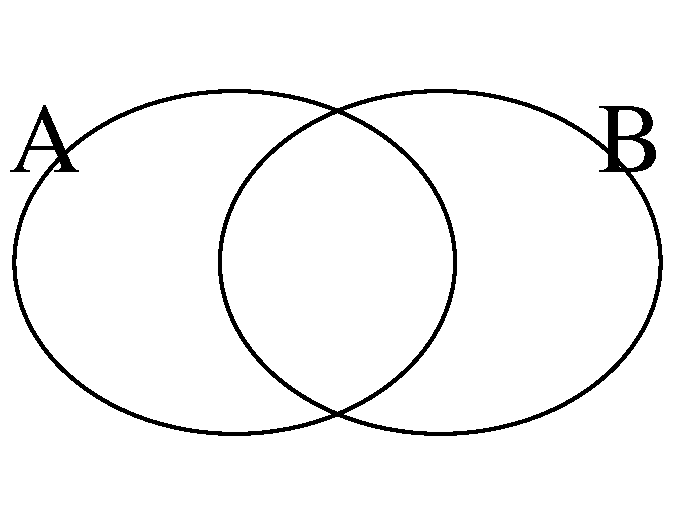
\includegraphics{Hypothesis_Test_Intro_files/figure-latex/unnamed-chunk-9-1.pdf}

\begin{verbatim}
## [1] 0.0002520202
\end{verbatim}

\begin{itemize}
\tightlist
\item
  Then the \(p\)-value is \(2\cdot 0.00025 = 0.0005\), so we reject the
  null hypothesis.
\item
  We can leave all the calculations to \textbf{R} by using
  \texttt{t.test}:
\end{itemize}

\begin{Shaded}
\begin{Highlighting}[]
\KeywordTok{t.test}\NormalTok{(statusquo }\OperatorTok{~}\StringTok{ }\NormalTok{sex, }\DataTypeTok{data =}\NormalTok{ Chile)}
\end{Highlighting}
\end{Shaded}

\begin{verbatim}
## 
##  Welch Two Sample t-test
## 
## data:  statusquo by sex
## t = 3.4786, df = 2678.7, p-value = 0.0005121
## alternative hypothesis: true difference in means is not equal to 0
## 95 percent confidence interval:
##  0.05849179 0.20962982
## sample estimates:
## mean in group F mean in group M 
##      0.06570627     -0.06835453
\end{verbatim}

\begin{itemize}
\tightlist
\item
  We recognize the \(t\)-score \(3.4786\) and the \(p\)-value
  \(0.0005\). The estimated degrees of freedom \(df = 2679\) is so large
  that we can not tell the difference between results obtained using
  \(z\)-score and \(t\)-score.
\end{itemize}

\subsection{Comparison of two means: confidence interval (independent
samples)}\label{comparison-of-two-means-confidence-interval-independent-samples}

\begin{itemize}
\tightlist
\item
  We have already found all the ingredients to construct a
  \textbf{confidence interval for \(\mu_2-\mu_1\)}:

  \begin{itemize}
  \tightlist
  \item
    \(d=\bar{y}_2-\bar{y}_1\) estimates \(\mu_2-\mu_1\).
  \item
    \(se_d=\sqrt{\frac{s_1^2}{n_1}+\frac{s_2^2}{n_2}}\) estimates the
    standard error of \(d\).
  \end{itemize}
\item
  Then: \[
    d\pm t_{crit}se_d
    \] is a confidence interval for \(\mu_2-\mu_1\).
\item
  The critical \(t\)-score, \(t_{crit}\) is chosen corresponding to the
  wanted confidence level. If \(n_1\) and \(n_2\) both are greater than
  30, then \(t_{crit} = 2\) yields a confidence level of approximately
  95\%.
\end{itemize}

\subsection{\texorpdfstring{Comparison of two means: paired \(t\)-test
(dependent
samples)}{Comparison of two means: paired t-test (dependent samples)}}\label{comparison-of-two-means-paired-t-test-dependent-samples}

\begin{itemize}
\tightlist
\item
  Experiment:

  \begin{itemize}
  \tightlist
  \item
    You choose 10 Netto stores at random, where you measure the average
    expedition time by the cash registers over some period of time.
  \item
    Now, new cash registers are installed in all 10 stores, and you
    repeat the experiment.
  \end{itemize}
\item
  It is interesting to investigate whether or not the new cash registers
  have changed the expedition time.
\item
  So we have 2 samples corresponding to old/new technology. In this case
  we have \textbf{dependent} samples, since we have 2 measurement in
  each store.
\item
  We use the following strategy for analysis:

  \begin{itemize}
  \tightlist
  \item
    For each store calculate \textbf{the change} in average expedition
    time when we change from old to new technology.
  \item
    The changes \(d_1,d_2,\ldots,d_{10}\) are now considered as
    \textbf{ONE} sample from a population with mean \(\mu\).
  \item
    Test the hypothesis \(H_0: \mu=0\) as usual (using a \(t\)-test for
    testing the mean as in the previous lecture).
  \end{itemize}
\end{itemize}

\begin{center}\rule{0.5\linewidth}{\linethickness}\end{center}

\subsubsection{Netto store example}\label{netto-store-example}

\begin{itemize}
\tightlist
\item
  Data is organized in a data frame with 2 variables, \texttt{before}
  and \texttt{after}, containing the average expedition time before and
  after installation of the new technology. Instead of doing manual
  calculations we let \textbf{R} perform the significance test (using
  \texttt{t.test} with \texttt{paired\ =\ TRUE} as our samples are
  paired/dependent):
\end{itemize}

\begin{Shaded}
\begin{Highlighting}[]
\NormalTok{Netto <-}\StringTok{ }\KeywordTok{read.delim}\NormalTok{(}\StringTok{"https://asta.math.aau.dk/datasets?file=Netto.txt"}\NormalTok{)}
\KeywordTok{head}\NormalTok{(Netto, }\DataTypeTok{n =} \DecValTok{3}\NormalTok{)}
\end{Highlighting}
\end{Shaded}

\begin{verbatim}
##     before    after
## 1 3.730611 3.440214
## 2 2.623338 2.314733
## 3 3.795295 3.586334
\end{verbatim}

\begin{Shaded}
\begin{Highlighting}[]
\KeywordTok{t.test}\NormalTok{(Netto}\OperatorTok{$}\NormalTok{before, Netto}\OperatorTok{$}\NormalTok{after, }\DataTypeTok{paired =} \OtherTok{TRUE}\NormalTok{)}
\end{Highlighting}
\end{Shaded}

\begin{verbatim}
## 
##  Paired t-test
## 
## data:  Netto$before and Netto$after
## t = 5.7204, df = 9, p-value = 0.0002868
## alternative hypothesis: true difference in means is not equal to 0
## 95 percent confidence interval:
##  0.1122744 0.2591578
## sample estimates:
## mean of the differences 
##               0.1857161
\end{verbatim}

\begin{itemize}
\tightlist
\item
  With a \(p\)-value of \(0.00029\) we reject that the expedition time
  is the same after installing new technology.
\end{itemize}

\section{Comparison of two
proportions}\label{comparison-of-two-proportions}

\subsection{Comparison of two
proportions}\label{comparison-of-two-proportions-1}

\begin{itemize}
\tightlist
\item
  We consider the situation, where we have two qualitative samples and
  we investigate whether a given property is present or not:

  \begin{itemize}
  \tightlist
  \item
    Let the proportion of population 1 which has the property be
    \(\pi_1\), which is estimated by \(\hat{\pi}_1\) based on a sample
    of size \(n_1\).
  \item
    Let the proportion of population 2 which has the property be
    \(\pi_2\), which is estimated by \(\hat{\pi}_2\) based on a sample
    of size \(n_2\).
  \item
    We are interested in the difference \(\pi_2-\pi_1\), which is
    estimated by \(d=\hat{\pi}_2-\hat{\pi}_1\).
  \item
    Assume that we can find the \textbf{estimated standard error}
    \(se_d\) of the difference.
  \end{itemize}
\item
  Then we can construct

  \begin{itemize}
  \tightlist
  \item
    an approximate confidence interval for the difference,
    \(\pi_2 - \pi_1\).
  \item
    a significance test.
  \end{itemize}
\end{itemize}

\subsection{Comparison of two proportions: Independent
samples}\label{comparison-of-two-proportions-independent-samples}

\begin{itemize}
\tightlist
\item
  In the situation where we have independent samples we know that \[
    se_d=\sqrt{se_1^2+se_2^2},
    \] where \(se_1\) and \(se_2\) are the estimated standard errors for
  the sample proportion in population 1 and 2, respectively.
\item
  We recall, that these are given by
  \(se=\sqrt{\frac{\hat{\pi}(1-\hat{\pi})}{n}}\), i.e. \[
    se_d = \sqrt{\frac{\hat{\pi}_1(1-\hat{\pi}_1)}{n_1}+\frac{\hat{\pi}_2(1-\hat{\pi}_2)}{n_2}}.
    \]
\item
  A (approximate) confidence interval for \(\pi_2-\pi_1\) is obtained by
  the usual construction:\\
  \[
    (\hat{\pi}_2-\hat{\pi}_1)\pm z_{crit}se_d,
    \] where the critical \(z\)-score determines the confidence level.
\end{itemize}

\subsection{Approximate test for comparing two proportions (independent
samples)}\label{approximate-test-for-comparing-two-proportions-independent-samples}

\begin{itemize}
\tightlist
\item
  We consider the null hypothesis \(H_0\): \(\pi_1=\pi_2\) (equivalently
  \(H_0: \pi_1 - \pi_2 = 0\)) and the alternative hypothesis \(H_a\):
  \(\pi_1 \neq \pi_2\).
\item
  Assuming \(H_0\) is true, we have a common proportion \(\pi\), which
  is estimated by \[
    \hat{\pi}=\frac{n_1\hat{\pi}_1+n_2\hat{\pi}_2}{n_1+n_2},
    \] i.e.~we aggregate the populations and calculate the relative
  frequency of the property (with other words: we estimate the
  proportion, \(\pi\), as if the two samples were one).
\item
  Rather than using the estimated standard error of the difference from
  previous, we use the following that holds under \(H_0\): \[
    se_0=\sqrt{\hat{\pi}(1-\hat{\pi})\left(\frac{1}{n_1}+\frac{1}{n_2}\right)}
    \]
\item
  The observed test statistic/\(z\)-score for \(H_0\) is then: \[
    z_{obs}=\frac{\hat{\pi}_2-\hat{\pi}_1}{se_0},
    \] which is evaluated in the standard normal distribution.
\item
  The \(p\)-value is calculated in the usual way.
\end{itemize}

\textbf{WARNING}: The approximation is only good, when \(n_1\hat{\pi},\
n_1(1-\hat{\pi}),\ n_2\hat{\pi},\ n_2(1-\hat{\pi})\) all are greater
than 5.

\subsection{Example: Approximate confidence interval and test for
comparing
proportions}\label{example-approximate-confidence-interval-and-test-for-comparing-proportions}

We return to the \texttt{Chile} dataset. We make a new binary variable
indicating whether the person intends to vote no or something else (and
we remember to tell \textbf{R} that it should think of this as a
grouping variable, i.e.~a \texttt{factor}):

\begin{Shaded}
\begin{Highlighting}[]
\NormalTok{Chile}\OperatorTok{$}\NormalTok{voteNo <-}\StringTok{ }\KeywordTok{relevel}\NormalTok{(}\KeywordTok{factor}\NormalTok{(Chile}\OperatorTok{$}\NormalTok{vote }\OperatorTok{==}\StringTok{ "N"}\NormalTok{), }\DataTypeTok{ref =} \StringTok{"TRUE"}\NormalTok{)}
\end{Highlighting}
\end{Shaded}

We study the association between the variables \texttt{sex} and
\texttt{voteNo}:

\begin{Shaded}
\begin{Highlighting}[]
\NormalTok{tab <-}\StringTok{ }\KeywordTok{tally}\NormalTok{( }\OperatorTok{~}\StringTok{ }\NormalTok{sex }\OperatorTok{+}\StringTok{ }\NormalTok{voteNo, }\DataTypeTok{data =}\NormalTok{ Chile, }\DataTypeTok{useNA =} \StringTok{"no"}\NormalTok{)}
\NormalTok{tab}
\end{Highlighting}
\end{Shaded}

\begin{verbatim}
##    voteNo
## sex TRUE FALSE
##   F  363   946
##   M  526   697
\end{verbatim}

This gives us all the ingredients needed in the hypothesis test:

\begin{itemize}
\tightlist
\item
  Estimated proportion of men that vote
  no:~\(\hat{\pi}_1=\frac{526}{526+697}=0.430\)
\item
  Estimated proportion of women that vote
  no:~\(\hat{\pi}_2=\frac{363}{363+946}=0.277\)
\item
  Estimated common
  proportion:~\(\hat{\pi}=\frac{1223 \times 0.430 + 1309 \times 0.277}{1309+1223}=\frac{526 + 363}{1309+1223}=0.351.\)
\item
  Estimated difference \(d=\hat{\pi}_2-\hat{\pi}_1=0.277-0.430=-0.153\)
\end{itemize}

Further,

\begin{itemize}
\tightlist
\item
  Standard error of difference:\\
  \(se_d=\sqrt{\frac{\hat{\pi}_1(1-\hat{\pi}_1)}{n_1}+\frac{\hat{\pi}_2(1-\hat{\pi}_2)}{n_2}}  = \sqrt{\frac{0.430(1-0.430)}{1223}+\frac{0.277(1-0.277)}{1309}}= 0.0188\).
\item
  Approximate 95\% confidence interval for
  difference:~\(d\pm  1.96se_d=(-0.190, -0.116)\).
\item
  Standard error of difference when \(H_0:\ \pi_1=\pi_2\) is true:\\
  \(se_0=\sqrt{\hat{\pi}(1-\hat{\pi})(\frac{1}{n_1}+\frac{1}{n_2})} = 0.0190\).
\item
  The observed test
  statistic/\(z\)-score:~\(z_{obs}=\frac{d}{se_0}=-8.06\). The test for
  \(H_0\) against \(H_a:  \pi_1\not=\pi_2\) yields a \(p\)-value that is
  practically zero, i.e.~we can reject that the proportions are equal.
\end{itemize}

\subsubsection{\texorpdfstring{Automatic calculation in
\textbf{R}}{Automatic calculation in R}}\label{automatic-calculation-in-r}

\begin{Shaded}
\begin{Highlighting}[]
\NormalTok{Chile2 <-}\StringTok{ }\KeywordTok{subset}\NormalTok{(Chile, }\OperatorTok{!}\KeywordTok{is.na}\NormalTok{(voteNo))}
\KeywordTok{prop.test}\NormalTok{(voteNo }\OperatorTok{~}\StringTok{ }\NormalTok{sex, }\DataTypeTok{data =}\NormalTok{ Chile2, }\DataTypeTok{correct =} \OtherTok{FALSE}\NormalTok{)}
\end{Highlighting}
\end{Shaded}

\begin{verbatim}
## 
##  2-sample test for equality of proportions without continuity
##  correction
## 
## data:  tally(voteNo ~ sex)
## X-squared = 64.777, df = 1, p-value = 8.389e-16
## alternative hypothesis: two.sided
## 95 percent confidence interval:
##  -0.1896305 -0.1159275
## sample estimates:
##    prop 1    prop 2 
## 0.2773109 0.4300899
\end{verbatim}

\subsection{Fisher's exact test}\label{fishers-exact-test}

\begin{itemize}
\tightlist
\item
  If
  \(n_1\hat{\pi},\ n_1(1-\hat{\pi}),\ n_2\hat{\pi},\ n_2(1-\hat{\pi})\)
  are not all greater than 5, then the approximate test cannot be
  trusted. Instead you can use Fisher's exact test:
\end{itemize}

\begin{Shaded}
\begin{Highlighting}[]
\KeywordTok{fisher.test}\NormalTok{(tab)}
\end{Highlighting}
\end{Shaded}

\begin{verbatim}
## 
##  Fisher's Exact Test for Count Data
## 
## data:  tab
## p-value = 1.04e-15
## alternative hypothesis: true odds ratio is not equal to 1
## 95 percent confidence interval:
##  0.4292768 0.6021525
## sample estimates:
## odds ratio 
##  0.5085996
\end{verbatim}

\begin{itemize}
\tightlist
\item
  Again the \(p\)-value is seen to be extremely small, so we definitely
  reject the null hypothesis of equal \texttt{voteNo} proportions for
  women and men.
\end{itemize}

\subsection{Agresti: Overview of comparison of two
groups}\label{agresti-overview-of-comparison-of-two-groups}

\includegraphics{https://asta.math.aau.dk/static-files/asta/img/agrSummaryTwoGroups.jpg}


\end{document}
